% This must be in the first 5 lines to tell arXiv to use pdfLaTeX, which is strongly recommended.
\pdfoutput=1
% In particular, the hyperref package requires pdfLaTeX in order to break URLs across lines.

\documentclass[11pt]{article}

% Change "review" to "final" to generate the final (sometimes called camera-ready) version.
% Change to "preprint" to generate a non-anonymous version with page numbers.
\usepackage{acl}

% Standard package includes
\usepackage{times}
\usepackage{latexsym}
\usepackage{subcaption}
\usepackage{lscape}
\usepackage{tikz}
\usepackage[edges]{forest}
\usetikzlibrary{trees, positioning, shapes, shadows, arrows.meta}
\usepackage{amsmath}
\usepackage{tabularray}
\usepackage{tabularx}
\definecolor{first}{RGB}{251,185,87}
\definecolor{second}{RGB}{115,186,161}
\definecolor{third}{RGB}{99,187,208}
\definecolor{fourth}{RGB}{210,217,122}
\definecolor{fifth}{RGB}{240,124,130}
\definecolor{sixth}{RGB}{209,194,211}
% For proper rendering and hyphenation of words containing Latin characters (including in bib files)
\usepackage[T1]{fontenc}
% For Vietnamese characters
% \usepackage[T5]{fontenc}
% See https://www.latex-project.org/help/documentation/encguide.pdf for other character sets

% This assumes your files are encoded as UTF8
\usepackage[utf8]{inputenc}

% This is not strictly necessary, and may be commented out,
% but it will improve the layout of the manuscript,
% and will typically save some space.
\usepackage{microtype}

% This is also not strictly necessary, and may be commented out.
% However, it will improve the aesthetics of text in
% the typewriter font.
\usepackage{inconsolata}

%Including images in your LaTeX document requires adding
%additional package(s)
\usepackage{graphicx}

% If the title and author information does not fit in the area allocated, uncomment the following
%
%\setlength\titlebox{<dim>}
%
% and set <dim> to something 5cm or larger.

\title{A Survey of Query Optimization in Large Language Models}

% Author information can be set in various styles:
% For several authors from the same institution:
% \author{Author 1 \and ... \and Author n \\
%         Address line \\ ... \\ Address line}
% if the names do not fit well on one line use
%         Author 1 \\ {\bf Author 2} \\ ... \\ {\bf Author n} \\
% For authors from different institutions:
% \author{Author 1 \\ Address line \\  ... \\ Address line
%         \And  ... \And
%         Author n \\ Address line \\ ... \\ Address line}
% To start a separate ``row'' of authors use \AND, as in
% \author{Author 1 \\ Address line \\  ... \\ Address line
%         \AND
%         Author 2 \\ Address line \\ ... \\ Address line \And
%         Author 3 \\ Address line \\ ... \\ Address line}

\author{Mingyang Song, Mao Zheng\\
	Machine Learning Platform Department, Tencent\\
	{\tt nickmysong@tencent.com} \\
}

%\author{
%  \textbf{First Author\textsuperscript{1}},
%  \textbf{Second Author\textsuperscript{1,2}},
%  \textbf{Third T. Author\textsuperscript{1}},
%  \textbf{Fourth Author\textsuperscript{1}},
%\\
%  \textbf{Fifth Author\textsuperscript{1,2}},
%  \textbf{Sixth Author\textsuperscript{1}},
%  \textbf{Seventh Author\textsuperscript{1}},
%  \textbf{Eighth Author \textsuperscript{1,2,3,4}},
%\\
%  \textbf{Ninth Author\textsuperscript{1}},
%  \textbf{Tenth Author\textsuperscript{1}},
%  \textbf{Eleventh E. Author\textsuperscript{1,2,3,4,5}},
%  \textbf{Twelfth Author\textsuperscript{1}},
%\\
%  \textbf{Thirteenth Author\textsuperscript{3}},
%  \textbf{Fourteenth F. Author\textsuperscript{2,4}},
%  \textbf{Fifteenth Author\textsuperscript{1}},
%  \textbf{Sixteenth Author\textsuperscript{1}},
%\\
%  \textbf{Seventeenth S. Author\textsuperscript{4,5}},
%  \textbf{Eighteenth Author\textsuperscript{3,4}},
%  \textbf{Nineteenth N. Author\textsuperscript{2,5}},
%  \textbf{Twentieth Author\textsuperscript{1}}
%\\
%\\
%  \textsuperscript{1}Affiliation 1,
%  \textsuperscript{2}Affiliation 2,
%  \textsuperscript{3}Affiliation 3,
%  \textsuperscript{4}Affiliation 4,
%  \textsuperscript{5}Affiliation 5
%\\
%  \small{
%    \textbf{Correspondence:} \href{mailto:email@domain}{email@domain}
%  }
%}

\begin{document}
\maketitle
\begin{abstract}
\textit{Query Optimization} (QO) refers to techniques aimed at enhancing the efficiency and quality of Large Language Models (LLMs) in understanding and answering queries, especially complex ones in scenarios like Retrieval-Augmented Generation (RAG). Specifically, RAG mitigates the limitations of LLMs by dynamically retrieving and leveraging up-to-date relevant information, which provides a cost-effective solution to the challenge of LLMs producing plausible but potentially inaccurate responses. Recently, as RAG evolves and incorporates multiple components that influence its performance, QO has emerged as a critical element, playing a pivotal role in determining the effectiveness of RAG's retrieval stage in accurately sourcing the necessary multiple pieces of evidence to answer queries correctly. In this paper,  we trace the evolution of QO techniques by summarizing and analyzing significant studies. Through an organized framework and categorization, we aim to consolidate existing QO techniques in RAG, elucidate their technological foundations, and highlight their potential to enhance the versatility and applications of LLMs.
\end{abstract}

\section{Introduction}
Large Language Models (LLMs) have made impressive achievements \cite{llm_survey}, yet they still encounter notable challenges, particularly in tasks that are domain-specific or heavily reliant on specialized knowledge \cite{survey1,survey2,survey3,survey4,survey5,survey6, survey7, survey8, survey9, survey10, survey11}. One prominent issue is their tendency to produce "hallucinations" when dealing with queries that surpass their training data or necessitate up-to-date information \cite{hallucination1, hallucination2}. To mitigate these challenges, Retrieval-Augmented Generation (RAG) enhances LLMs by retrieving relevant segments, effectively diminishing the production of factually incorrect content. The widespread integration of RAG into LLMs has established it as a crucial technology for the advancement of query solvers and has improved the suitability of LLMs for practical, real-world applications.

\begin{figure}
	\centering
	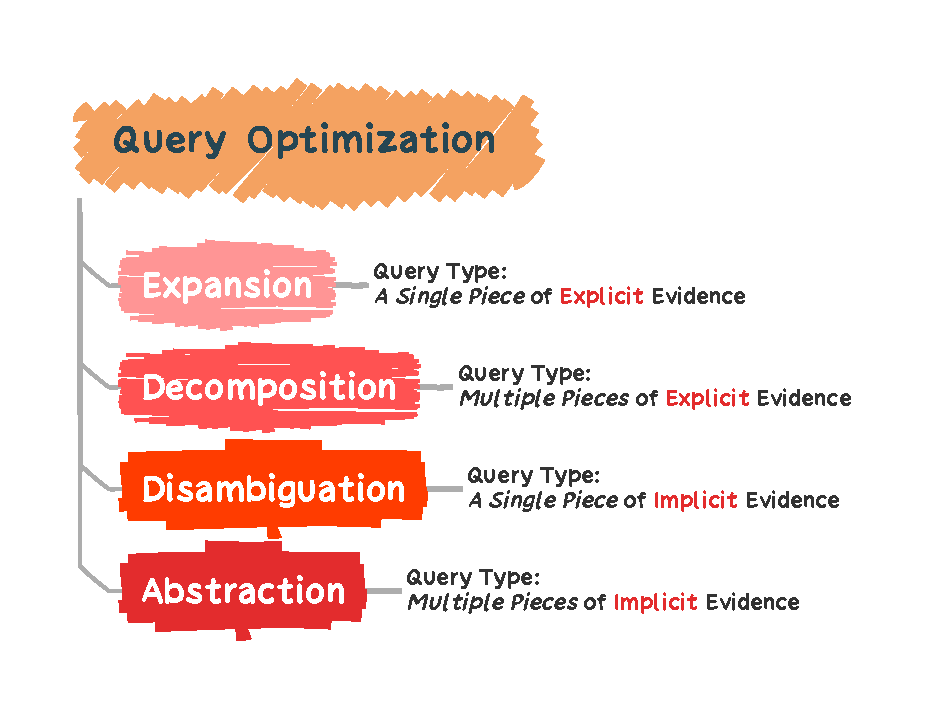
\includegraphics[scale=0.53]{figure/QueryOptimizationAbs.pdf}
	\caption{Four atomic operations in QO.}
	\label{intro}
\end{figure}

Since \citet{2020rag} introduced RAG, the field has advanced rapidly, particularly with the emergence of models like ChatGPT. Despite these developments, there is a significant gap in the literature—a thorough analysis of RAG's underlying mechanisms and the progress made in subsequent studies is lacking. Furthermore, the field is characterized by fragmented research focuses and inconsistent terminology for similar methods, which leads to confusion.



RAG typically involves several core concepts, including but not limited to query optimization, information retrieval, and response generation \cite{survey3, survey4, survey5}. Among these, query optimization plays a crucial role in directly determining the relevance of the retrieved information and consequently impacts the quality of the final response. Although query optimization in retrieval-augmented large language models (LLMs) has experienced rapid growth, there has been a lack of systematic synthesis to clarify its broader trajectory. This survey endeavors to fill this gap by mapping out the query optimization process in retrieval-augmented LLMs, charting its evolution, and anticipating future developments.
We consider both technical paradigms and research methods, summarizing four main approaches identified in recent LLM-based RAG studies: \textit{Expansion}, \textit{Disambiguation}, \textit{Decomposition}, and \textit{Abstraction}, as shown in Figure~\ref{intro}, and then categorize the corresponding atomic operations for query optimization and map them accordingly. We classify the difficulty of most queries into four types: those that can be solved with a single piece of explicit evidence, those requiring multiple pieces of explicit evidence, those solvable with a single piece of implicit evidence, and those needing multiple pieces of implicit evidence. We then map these queries to different optimization operations respectively for ease of explanation, as shown in Figure~\ref{intro_detail}. Next, we briefly introduce each type of query and the corresponding optimization method, as illustrated in Figure~\ref{fig:qo tax}.

Overall, this paper aims to meticulously compile and categorize the foundational technical concepts, historical developments, and the range of query optimization methodologies and applications that have emerged since the advent of LLMs. It is designed to equip readers and professionals with a detailed and structured understanding of query optimization in retrieval-augmented LLMs, illuminating the evolution of these techniques and speculating on upcoming trends and innovations.



Query optimization techniques summarized in this paper may involve multiple scenarios, including but not limited to retrieval-augmented generation, question answering, etc. Therefore, we uniformly adopt the term "query" to represent terms such as "query", "question", and "problem" in the subsequent content.

Additionally, this survey is organized as follows: Section~\ref{Stratification} introduces the stratification of query optimization. The subsequent sections delve into key techniques in query optimization: Section~\ref{Expansion} explores query expansion, which is further divided into internal expansion (Section~\ref{Internal}) and external expansion (Section~\ref{External}). Section~\ref{Decomposition} discusses query decomposition. Section~\ref{Disambiguation} and Section~\ref{Abstraction} focus on disambiguation and abstraction. Section~\ref{Challenges} addresses the challenges and future directions in this field. Finally, the conclusion and limitations are presented in Section~\ref{Conclusion} and Section~\ref{Limitations}.

\begin{figure*}[h]
	\centering
	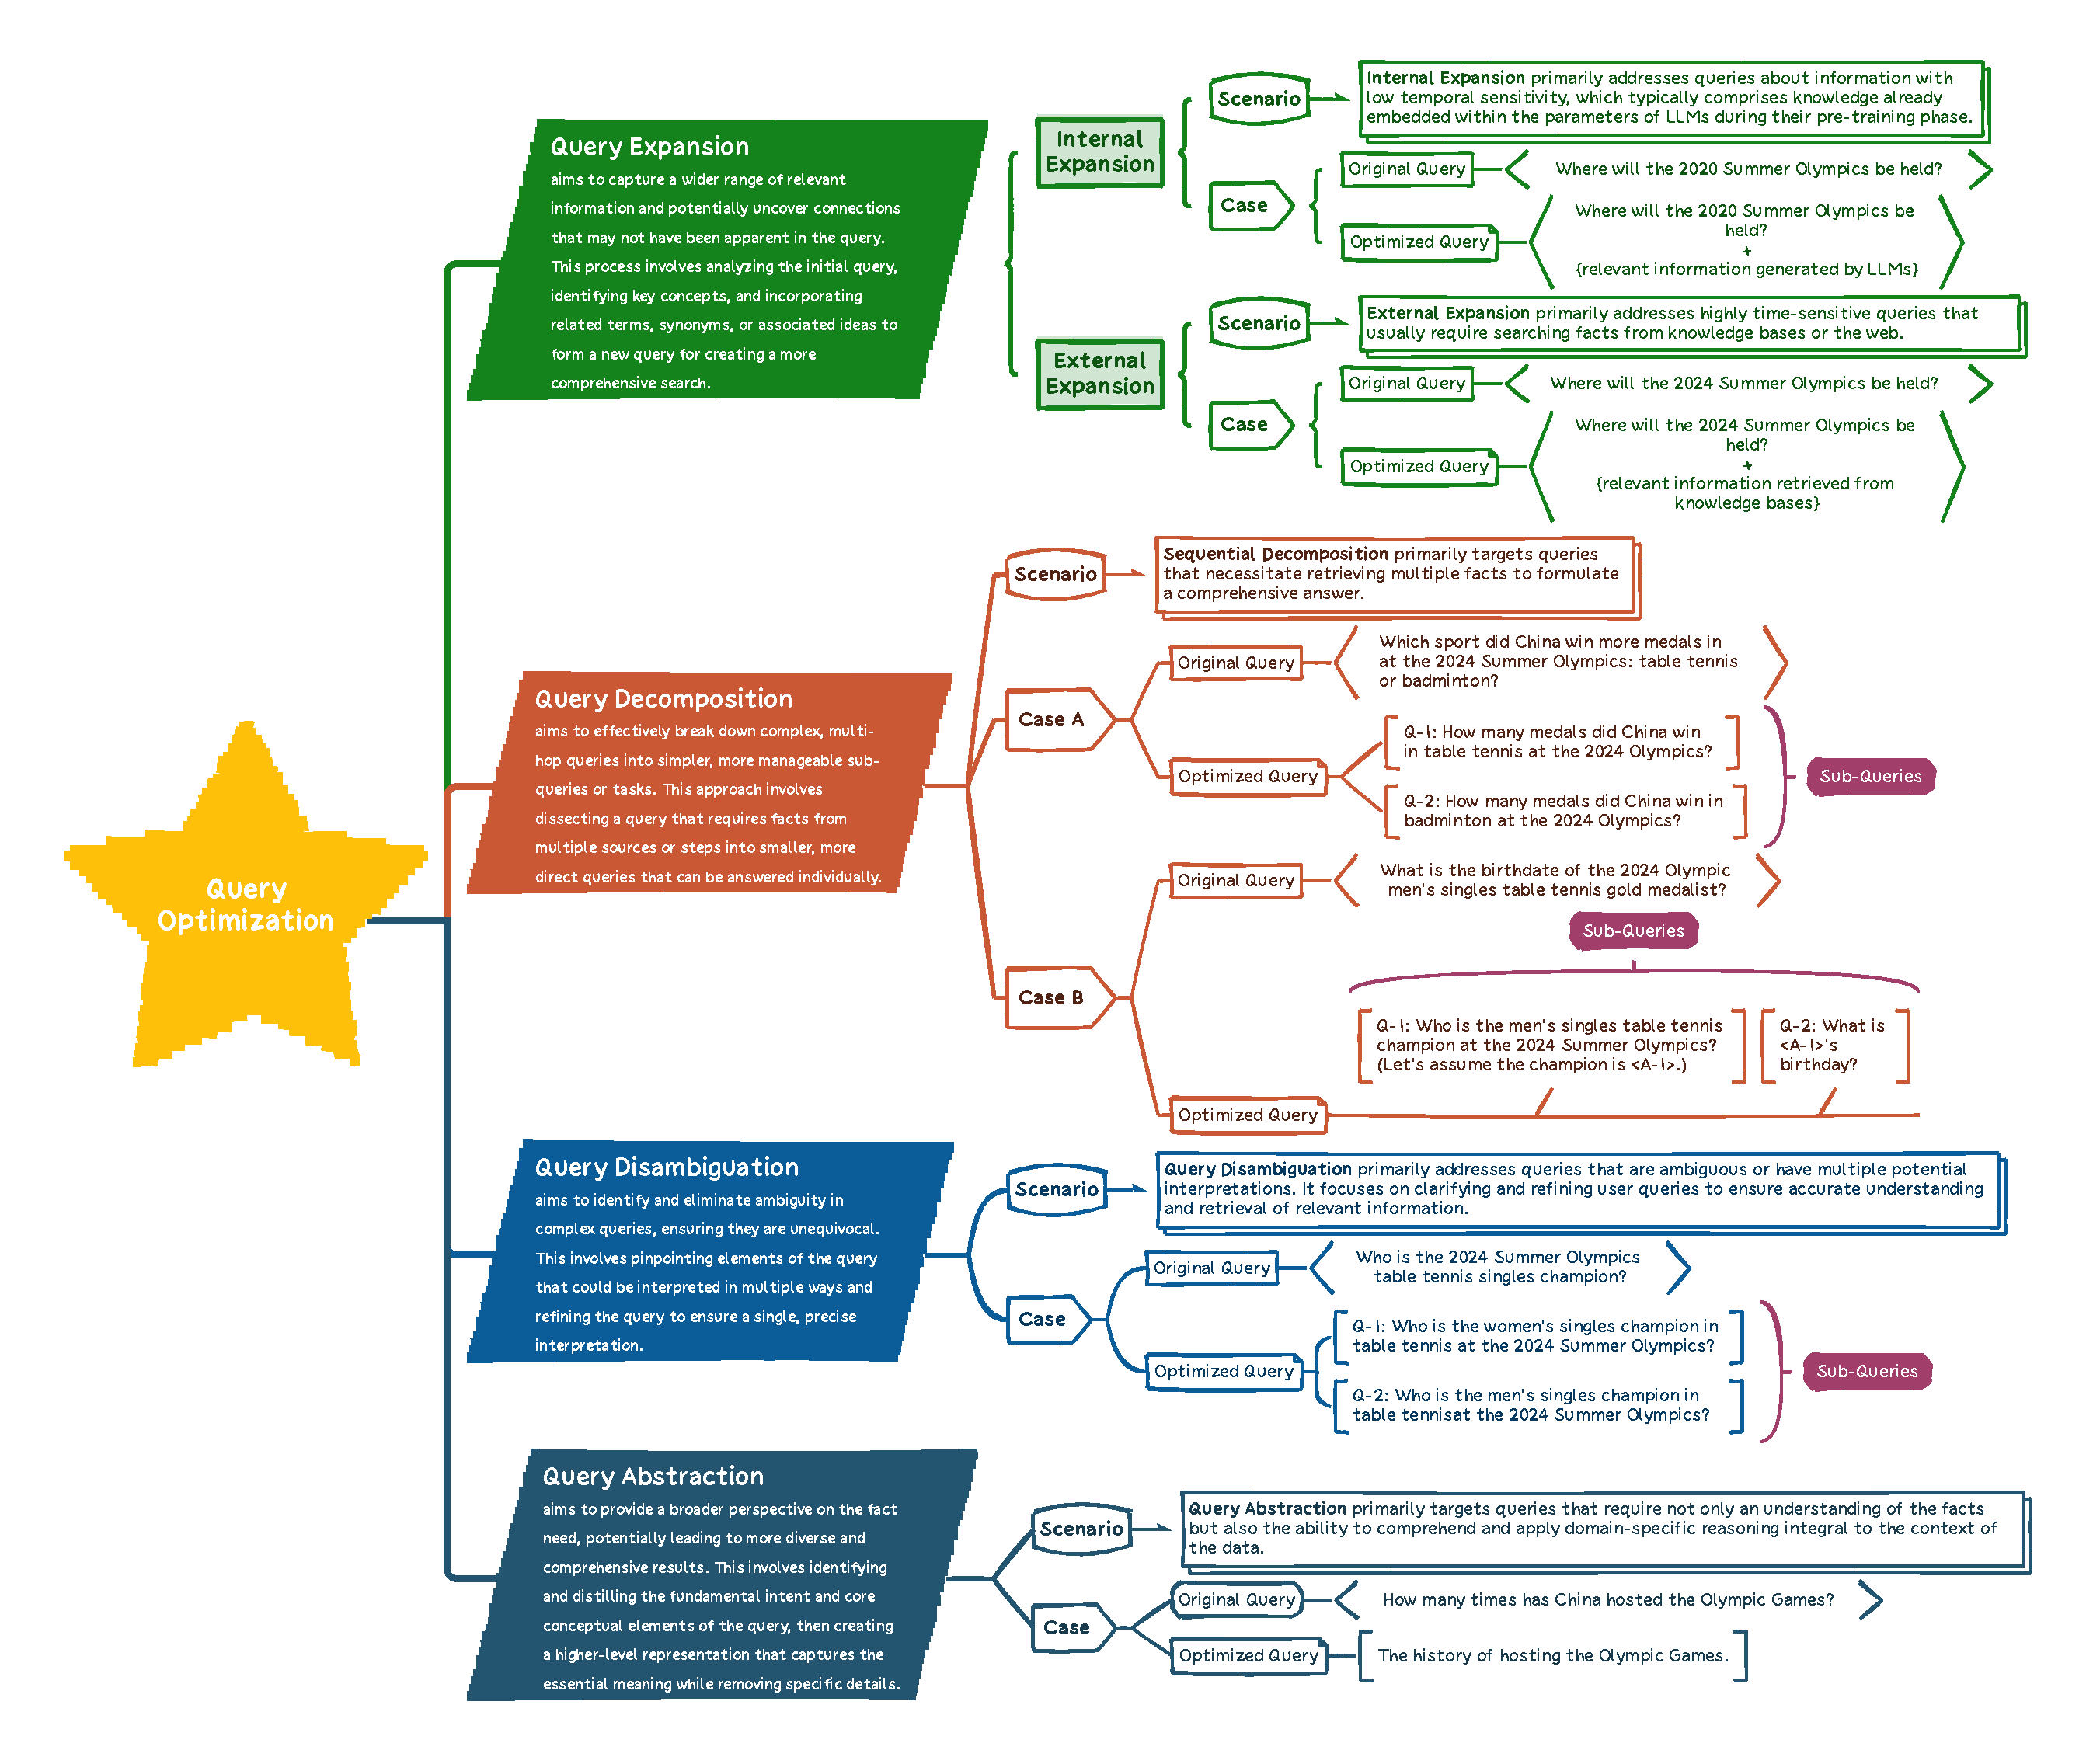
\includegraphics[scale=0.36]{figure/QueryOptimizationIntro.pdf}
	\caption{Classification of query optimization techniques in detail.}
	\label{intro_detail}
\end{figure*}



\begin{figure*}[t]
	\centering
	\tikzset{
		root/.style   = {align=center, fill=first, text width=7cm, font=\Large},
		xnode/.style = {align=center, fill=second, text width=5cm, font=\Large},
		ynode/.style = {align=center, fill=third, text width=5cm, font=\Large},
		znode/.style = {align=center, fill=sixth, text width=5cm, font=\Large},
		pnode/.style = {align=center, fill=fourth, text width=5cm, font=\normalsize},
		dnode/.style = {align=center, fill=second, text width=5cm, font=\Large},
		edge from parent/.style={draw=black, very thick, edge from parent fork south},
	}
	\resizebox{\textwidth}{!}{%
		\begin{forest}
			for tree={
				grow=south,
				growth parent anchor=south,
				parent anchor=south,
				child anchor=north,
				draw,
				minimum height = 1cm,
				rounded corners=10pt,
				drop shadow,
				node options={align=center,},
				text width=2.5cm,
				l sep=10mm,
				s sep=3mm,
				edge={ultra thick, draw=black},
				tier/.wrap pgfmath arg={tier #1}{level()},
				edge path={
					\noexpand\path [\forestoption{edge}, ultra thick]
					(!u.parent anchor) -- +(0,-15pt) -|   
					(.child anchor)\forestoption{edge label};
				},
			}
			[\textsc{Query Optimization}, root, for tree={parent anchor=south}
		      [\textsc{Expansion}, dnode, for tree={parent anchor=south}
			[\textsc{Internal}, znode, for tree={parent anchor=south}
			[{\textsc{GenQREnsemble} \\\cite{GenQREnsemble} \\\textsc{GuideCQR} \\\cite{GuideCQR} \\\textsc{Query2doc} \\\cite{Query2doc} \\\textsc{GQE} \\\cite{GQE} \\\textsc{CSQE} \\\cite{CSQE} \\\textsc{MUGI} \\\cite{MUGI} \\\textsc{EQE} \\\cite{EQE} \\\textsc{HyDE} \cite{HyDE} \\\textsc{FLARE} \\\cite{FLARE} \\\textsc{GenRead} \\\cite{GenRead} \\\textsc{InteR} \\\cite{InteR} \\\textsc{EAR} \\\cite{EAR} \\\textsc{MILL} \\\cite{MILL} 
			}, pnode]]
			[\textsc{External}, znode, for tree={parent anchor=south}
			[{\textsc{MUGI} \\\cite{MUGI} \\\textsc{KnowledGPT} \\\cite{KnowledGPT} \\\textsc{Promptagator} \\\cite{Promptagator} \\\textsc{RARG} \\\cite{RARG} \\\textsc{DRAGIN} \\\cite{DRAGIN} \\\textsc{EWEK-QA} \\\cite{EWEK-QA} \\\textsc{BlendFilter} \\\cite{BlendFilter} \\\textsc{ReFeed} \\\cite{ReFeed} \\\textsc{Query2Expand} \\\cite{Query2Expand} \\\textsc{DR-RAG} \\\cite{DR-RAG} \\\textsc{CoV-RAG} \\\cite{CoV-RAG} \\\textsc{MILL} \\\cite{MILL} \\\textsc{LameR} \\\cite{LameR} 
			}, pnode]]] 
            [\textsc{Decomposition}, dnode, for tree={parent anchor=south}
			[{\textsc{RAG-Star} \\\cite{RAG-Star} \\\textsc{Plan$\times$RAG} \\\cite{plantimesrag} \\\textsc{ConTReGen} \\\cite{ConTReGen} \\\textsc{RichRAG} \\\cite{RichRAG}  \\\textsc{ALTER} \\\cite{ALTER} \\\textsc{LPKG} \\\cite{LPKG} \\\textsc{RA-ISF} \\\cite{RA-ISF} \\\textsc{Think-then-Act} \\\cite{Think-then-Act} \\\textsc{AutoPRM} \\\cite{AutoPRM} \\\textsc{RQ-RAG} \\\cite{RQ-RAG} \\\textsc{QDMR} \\\cite{QDMR} \\\textsc{Rewrite-Retrieve-Read} \\\cite{Rewrite-Retrieve-Read}\\\textsc{rStar} \\\cite{rStar} \\\textsc{Least-to-Most} \\\cite{Least-to-Most} \\\textsc{HiRAG} \\\cite{HiRAG} \\\textsc{CoK} \cite{CoK} \\\textsc{DSP} \cite{Demonstrate-Search-Predict} \\\textsc{Self-Ask} \\\cite{Self-Ask} \\\textsc{DecomP} \\\cite{DecomP} \\\textsc{ICAT} \\\cite{ICAT} \\\textsc{Plan-and-Solve} \\\cite{Plan-and-Solve} \\\textsc{IM-RAG} \\\cite{IM-RAG} \\\textsc{MQA-KEAL} \\\cite{MQA-KEAL} \\\textsc{ReAct} \\\cite{ReAct} \\\textsc{REAPER} \\\cite{REAPER}  
			}, pnode]]
			[\textsc{Disambiguation}, ynode, for tree={parent anchor=south}
			[{\textsc{rStar} \\\cite{rStar} \\\textsc{RQ-RAG} \\\cite{RQ-RAG} \\\textsc{RaFe} \\\cite{RaFe} \\\textsc{ToC} \\\cite{ToC} \\\textsc{BEQUE} \\\cite{BEQUE}  \\\textsc{AdaQR} \\\cite{AdaQR} \\\textsc{CHIQ} \\\cite{CHIQ} \\\textsc{EchoPrompt} \\\cite{EchoPrompt} \\\textsc{MaFeRw} \\\cite{MaFeRw} \\\textsc{InfoCQR} \\\cite{InfoCQR} \\\textsc{Natural-Program} \\\cite{Natural-Program} 
			}, pnode]]
             [\textsc{Abstraction}, ynode, for tree={parent anchor=south}
			[{\textsc{SimGRAG} \\\cite{SimGRAG} \\\textsc{CoA} \\\cite{CoA} \\\textsc{Crafting-the-Path} \\\cite{Crafting-the-Path} \\\textsc{AbsInstruct} \\\cite{AbsInstruct} \\\textsc{AoT} \\\cite{AoT} \\\textsc{AbsPyramid} \\\cite{AbsPyramid} \\\textsc{Meta-Reasoning} \\\cite{Meta-Reasoning} \\\textsc{Conceptualization-Abstraction} \\\cite{Conceptualization-Abstraction} \\\textsc{MA-RIR} \\\cite{MA-RIR} \\\textsc{RuleRAG} \\\cite{RuleRAG} \\\textsc{StepBack} \\\cite{StepBack} 
			}, pnode]]	
			]
		\end{forest}
	}
	\caption{Taxonomy tree of core techniques of query optimization.}
	\label{fig:qo tax}
\end{figure*}



\section{Stratification of Query Optimization}\label{Stratification}
Query optimization is crucial for enhancing the effectiveness and precision of retrieval-augmented generation using large language models. By refining users' original queries, this process addresses several challenges, including ambiguous semantics, complex requirements, and discrepancies in relevance between the query and target documents. Effective query optimization demands a profound understanding of user intent and query context, especially when dealing with intricate or multifaceted inquiries. When implemented successfully, it significantly improves problem-solving performance, substantially impacting the quality of the model's generated outputs. Ultimately, this enhancement in query processing leads to more accurate and contextually appropriate responses, elevating the overall user experience and increasing the utility of LLMs across various applications.

\subsection{Query Expansion}\label{Expansion}
Query Expansion techniques \cite{query_expansion_survey1} are critical in enhancing the performance of retrieval-augmented generation, particularly when integrated with LLMs \cite{query_expansion_survey2}. Based on the different sources of knowledge, we broadly categorize it into internal expansion and external expansion. The former focuses on maximizing the value of existing information in the original query or the used LLM without relying on external knowledge sources., while the latter introduces supplementary data from outside sources (e.g., Web or Knowledge base) to fill gaps, provide additional context, or broaden the scope of the content.

\subsubsection{Internal Expansion}\label{Internal}
In recent years, researchers have developed various query expansion techniques to enhance information retrieval systems by leveraging LLMs. One of the early approaches is \textsc{GenRead} \cite{GenRead}, which employs a well-designed instruction to prompt LLMs to generate contextual documents based on the initial query. These generated documents are then read by the LLM to produce the final response, effectively bridging the gap between query understanding and answer generation.

Building upon the concept of query expansion, \textsc{Query2Doc} \cite{Query2doc} introduces a simple yet effective approach to improve both sparse and dense retrieval systems. By generating pseudo-documents through the few-shot prompting of LLMs, the original query is expanded with these generated documents. Since LLMs are trained on web-scale text corpora, these pseudo-documents often contain highly relevant information that aids in disambiguating queries and guiding retrievers toward more pertinent results.

In a similar vein, \textsc{ReFeed} \cite{ReFeed} tackles LLM limitations efficiently and cost-effectively by first generating initial outputs. It then retrieves relevant information from large document collections using a retrieval model and incorporates this information into the in-context demonstration to refine the output. This iterative process enhances the quality of the final response by grounding it in retrieved data.

\textsc{InteR} \cite{InteR} presents an interactive retrieval framework where retrieval models expand the knowledge within queries by utilizing LLM-generated knowledge collections. Concurrently, LLMs enhance prompt formulation by leveraging retrieved documents, creating a synergistic loop between the retrieval models and the LLMs for improved information access.

Approaching the challenge from a different angle, \textsc{HyDE} \cite{HyDE} employs a zero-shot prompt with a language model to generate a hypothetical document that captures relevant patterns, even if it contains "hallucinations." An unsupervised contrastive encoder then encodes this document into an embedding vector to identify a neighborhood in the corpus embedding space. By retrieving similar real documents based on vector similarity, \textsc{HyDE} grounds the generated content to the actual corpus, with the encoder's dense bottleneck filtering out inaccuracies.
\textsc{FLARE} \cite{FLARE} introduces an iterative anticipation mechanism where, based on the original query, it predicts future content and retrieves relevant information to enhance retrieval performance. If the generated temporary next sentence contains low-confidence tokens, \textsc{FLARE} treats it as a new query to retrieve additional documents, repeating this process until a satisfactory answer is obtained.

Expanding on query generation, \textsc{MILL} \cite{MILL} proposes a query–query–document generation approach that leverages the zero-shot reasoning capabilities of LLMs to produce diverse sub-queries and corresponding documents. A mutual verification process then synergizes the generated and retrieved documents, leading to optimal expansion and comprehensive retrieval results.

To further refine retrieval performance, \textsc{GenQREnsemble} \cite{GenQREnsemble} suggests an ensemble-based prompting technique that uses paraphrases of a zero-shot instruction to generate multiple sets of keywords. By combining these keyword sets, the method enhances retrieval efficacy through diversity and redundancy.

Lastly, \textsc{ERRR} \cite{ERRR} emphasizes the extraction of parametric knowledge from LLMs and the refinement of these queries using a specialized query optimizer. This approach ensures that only the most pertinent information is retrieved, which is essential for generating accurate and relevant responses.

\subsubsection{External Expansion}\label{External}
External Expansion is a sophisticated process that significantly enhances document content by seamlessly integrating pertinent information from diverse external sources. This methodology augments the overall context, depth, and accuracy of the document corpus. The enrichment process involves strategically incorporating authoritative facts, up-to-date data points, and relevant contextual knowledge derived from a wide array of external datasets, knowledge bases, and curated information repositories.

LameR \cite{LameR} augments a query with its potential answers by prompting LLMs with a combination of the query and the question's in-domain candidates. These candidates, regardless of whether they are correct or incorrect, are obtained through a standard retrieval procedure on the target collection.
GuideCQR \cite{GuideCQR} refines queries for conversational query reformulation by leveraging key information from the initially retrieved documents.
CSQE \cite{CSQE} promotes the incorporation of knowledge embedded within the corpus and leverages the relevance-assessing capabilities of LLMs to systematically identify pivotal sentences in the initially retrieved documents. These corpus-derived texts are then used to expand the query, along with LLM-empowered expansions, enhancing the relevance prediction between the query and the target documents.
MUGI \cite{MUGI} explores and leverages LLMs to generate multiple pseudo references, integrating them with queries to enhance both sparse and dense retrievers.

\subsection{Question Decomposition}\label{Decomposition}
For complex queries, simply searching with the original query often fails to retrieve adequate information. It is crucial for LLMs to first decompose such queries into simpler, answerable sub-queries, and then search for information relevant to these sub-components. By integrating the responses to these sub-queries, LLMs are able to construct a comprehensive response to the original query.

One such method is the Demonstrate Search Predict (\textsc{DSP}) framework \cite{Demonstrate-Search-Predict}, which relies on passing natural language texts through sophisticated pipelines between an LLM and a retrieval model (RM). \textsc{DSP} can express high-level programs that bootstrap pipeline-aware demonstrations, search for relevant passages, and generate grounded predictions, systematically breaking down problems into small transformations that the LLM and RM can handle more reliably.

Similarly, techniques like \textsc{Least-to-Most} \cite{Least-to-Most} prompting utilize few-shot prompts to first decompose a complex problem into a series of simpler subproblems and then solve them in sequence. \textsc{Plan-and-Solve} \cite{Plan-and-Solve} prompting involves devising a plan to divide the entire task into smaller subtasks and then carrying out these subtasks according to the plan. These approaches emphasize the importance of decomposition in handling complex queries, allowing models to process each component effectively.

\textsc{SELF-ASK} \cite{Self-Ask} introduces the concept of the compositionality gap, which describes the fraction of compositional queries that the model answers incorrectly out of all the compositional queries for which the model answers the sub-queries correctly. This highlights the challenges LLMs face in integrating answers from sub-queries to solve more complex queries.

To address retrieval challenges, approaches like \textsc{EAR} \cite{EAR} apply a query expansion model to generate a diverse set of queries, using a query reranker to select those that could lead to better retrieval results. Correction of Knowledge (\textsc{CoK}) \cite{CoK} first proposes and prepares several preliminary rationales and answers while identifying the relevant knowledge domains. If there is no majority consensus among the answers, \textsc{CoK} corrects the rationales step by step by adapting knowledge from the identified domains, serving as a better foundation for the final response consolidation.

In the realm of transferring abilities to LLMs, \textsc{ICAT} \cite{ICAT} induces reasoning capabilities without any LLM fine-tuning or manual annotation of in-context samples. It transfers the ability to decompose complex queries into simpler ones or generate step-by-step rationales by carefully selecting from available data sources of related tasks.

\textsc{ReAct} \cite{ReAct} introduces a paradigm to combine reasoning and acting with LLMs for solving diverse language reasoning and decision-making tasks. \textsc{ReAct} prompts LLMs to generate both verbal reasoning traces and actions on a task in an interleaved manner. This allows the model to perform dynamic reasoning to create, maintain, and adjust high-level plans for acting ("reason to act"), while also interacting with external environments (e.g., Wikipedia) to incorporate additional information into reasoning ("act to reason").

Approaches like \textsc{AutoPRM} \cite{AutoPRM} and \textsc{RA-ISF} \cite{RA-ISF} employ query decomposition to handle complex queries. \citet{AutoPRM} first decomposes complex problems into more manageable sub-queries with a controllable granularity switch, then sequentially apply reinforcement learning to iteratively improve the sub-query solver. \citet{RA-ISF} mitigates the impact of irrelevant prompts by iteratively addressing sub-queries while integrating text relevance with self-knowledge answering capabilities. The process involves breaking down the initial multi-turn query into single-turn queries, addressing each sub-task independently, and then synthesizing these responses to resolve the initial query.

Other methods enhance models by equipping them with capabilities for explicit rewriting, decomposition, and disambiguation, such as \textsc{RQ-RAG}. \textsc{LPKG} \cite{LPKG} enhances the query planning capabilities of LLMs by grounding predefined patterns in an open-domain knowledge graph to extract numerous instances, which are then verbalized into complex queries and corresponding sub-queries in natural language.

Techniques like \textsc{ALTER} \cite{ALTER} and \textsc{IM-RAG} \cite{IM-RAG} focus on enhancing retrieval and reasoning processes. Specifically, \textsc{ALTER} employs a question augmentor to enhance the original question by generating multiple sub-queries, each examining the original question from different perspectives, for handling complex table reasoning tasks. \textsc{IM-RAG} introduces a Refiner that improves the outputs from the Retriever, effectively bridging the gap between the Reasoner and information retrieval modules with varying capabilities and fostering multi-round communications.

\textsc{REAPER} \cite{REAPER}, a reasoning-based planner, is designed for efficient retrieval required for complex queries. Using a single and smaller LLM, REAPER generates a plan that includes the tools to call, the order in which they should be called, and the arguments for each tool.

Building on previous studies, \textsc{HiRAG} \cite{HiRAG} decomposes the original query into multi-hop queries. Each sub-query is answered based on retrieved knowledge, and the answers are then integrated using the Chain-of-Thought (CoT) approach to derive the final answer. \textsc{MQA-KEAL} \cite{MQA-KEAL} stores knowledge edits as structured knowledge units in external memory. To solve multi-hop queries, it first uses task decomposition to break the query into smaller sub-problems. For each sub-problem, it iteratively queries the external memory and/or the target LLM to generate the final response.

Recent methods like \textsc{RichRAG} \cite{RichRAG} and \textsc{ConTReGen} \cite{ConTReGen} further improve the retrieval process. \textsc{RichRAG} introduces a sub-aspect explorer to dissect input queries and uncover their latent facets. This is integrated with a multi-faceted retriever, which curates a diverse corpus of external documents pertinent to these identified sub-aspects to answer queries. \textsc{ConTReGen} proposes a context-driven, tree-structured retrieval approach to enhance the depth and relevance of retrieved content. It incorporates a hierarchical, top-down in-depth exploration of query facets with a systematic bottom-up synthesis, ensuring comprehensive coverage and coherent integration of multifaceted information.

\textsc{Plan×RAG} \cite{plantimesrag} formulates a comprehensive reasoning plan represented as a directed acyclic graph (DAG). This reasoning DAG decomposes the main query into interrelated atomic sub-queries, providing a computational structure that enables efficient information sharing between sub-queries. \textsc{RAG-Star} \cite{RAG-Star} seamlessly integrates retrieved information to guide a tree-based deliberative reasoning process, leveraging the inherent knowledge of LLMs. By utilizing Monte Carlo Tree Search, \textsc{RAG-Star} iteratively plans intermediate sub-queries and generates answers for reasoning based on the capabilities of the LLM itself.


\subsection{Query Disambiguation}\label{Disambiguation}
For ambiguous queries with multiple possible answers, relying solely on the original query for information retrieval is inadequate. To deliver complete and nuanced responses, LLMs must learn to clarify the query by identifying the user's intent and then formulate a more targeted search query. After gathering relevant information, LLMs can provide a detailed and comprehensive response. There are mainly two types of approaches for query disambiguation. One is when the query itself is ambiguous, and the other is for multi-turn queries, where it's necessary to rewrite the query by incorporating historical dialogue content to achieve disambiguation \cite{BEQUE, RaFe}.

\citet{Natural-Program} early introduces a deductive reasoning format based on the natural language that decomposes the reasoning verification process into a series of step-by-step subprocesses. Each subprocess receives only the necessary context and premises, allowing LLMs to generate precise reasoning steps that are rigorously grounded on prior ones. This approach empowers language models to conduct reasoning self-verification sequentially, significantly enhancing the rigor and trustworthiness of the generated reasoning steps.

Building upon the refinement of model reasoning, \textsc{EchoPrompt} \cite{EchoPrompt} introduces a query-rephrasing subtask by employing prompts like “\textit{Let’s repeat the query and also think step by step.}”. This encourages the model to restate the query in its own words before engaging in reasoning, ensuring better understanding and consistency. Importantly, the prompt used for answer extraction remains consistent across all zero-shot methodologies.
\textsc{ToC} \cite{ToC} recursively builds a tree of disambiguations for ambiguous queries by utilizing few-shot prompting and external knowledge. It retrieves relevant facts to generate a comprehensive long-form answer based on this tree, thus providing more accurate and detailed responses.
\textsc{InfoCQR} \cite{InfoCQR} introduces a novel "rewrite-then-edit" framework, where LLMs first rewrite the original query and then revise the rewritten query to eliminate ambiguities. The well-designed instructions independently guide the LLMs through the rewriting and editing tasks, resulting in more informative and unambiguous queries.

To further manipulate the disambiguated query, \textsc{AdaQR} \cite{AdaQR} proposes a novel preference optimization approach, which aims to tailor rewriters to better suit retrievers by utilizing conversation answers to model retrievers’ preferences. Specifically, the trained rewriter generates several rewrites, which are then used as queries to retrieve passages from a target retriever. Then, \textsc{AdaQR} calculates the conditional probability of the answer given each retrieved passage and the conversation, obtaining the marginal probability of the answer by marginalizing over the set of passages. This marginal probability serves as a reward that quantifies the retrievers’ preferences over rewrites and pairs these rewrites based on their rewards to optimize the trained rewriter using direct preference optimization.

\textsc{MaFeRw} \cite{MaFeRw} improves the RAG performance by integrating multi-aspect feedback from both the retrieved documents and the generated responses as rewards to explore the optimal query rewriting strategy. This approach leverages comprehensive feedback to enhance the effectiveness of query rewriting. \textsc{CHIQ} leverages the NLP capabilities of LLMs, such as resolving coreference relations and expanding context, to reduce ambiguity in conversational history. This enhancement improves the relevance of the generated search queries. We investigate various methods for integrating refined conversational history into existing frameworks, including ad-hoc query rewriting, generating pseudo-supervision signals for fine-tuning query rewriting models, and combining both approaches.

\section{Query Abstraction}\label{Abstraction}
For complex multi-hop queries, sequential decomposition may not yield accurate answers and can even complicate the query further. Humans often step back and perform abstractions to arrive at high-level principles to solve complex queries, reducing the chance of making errors in the intermediate reasoning steps \cite{StepBack}.

\textsc{Step-Back} \cite{StepBack} manipulates the initial query using meticulously designed prompts that steer the LLM's reasoning process. This ensures that the outputs are more closely aligned with the idea behind the original query, especially for tasks requiring complex reasoning.
Building upon the idea of guiding reasoning through abstraction, \cite{Conceptualization-Abstraction} requires LLMs to engage in conceptual reasoning with abstract queries, producing solutions within a verifiable symbolic space. This promotes a deeper understanding and handling of abstract concepts.
\textsc{CoA} \cite{CoA} abstracts the general CoT reasoning into a reasoning chain with abstract variables. This enables LLMs to solve queries by utilizing domain-specialized tools, such as calculation results from a calculator or relevant articles retrieved from web search engines.

Similarly, \textsc{AoT} \cite{AoT} utilizes an abstract skeletal framework to structure the entire reasoning process, potentially unlocking the key to eliciting abstract reasoning. Unlike the unconstrained CoT, the \textsc{AoT} format explicitly integrates different levels of abstraction throughout the reasoning process. At each higher level, the abstraction is a distilled version of the lower level, containing fewer concrete details while clearly stating the objective and functionality of each reasoning step.
In addition, \citet{Crafting-the-Path} generates a higher level of abstraction information that serves as the contextual background for the existing query. This approach enriches the direct information about the query object within the initial query, providing a more comprehensive understanding.

Focusing on multi-faceted queries, \textsc{MA-RIR} \cite{MA-RIR} defines a query aspect as a sub-span of a multi-aspect query that represents a distinct topic or facet within the query. This allows for more focused and effective reasoning across different aspects of a complex query.
To further improve reasoning efficiency and accuracy, \textsc{Meta-Reasoning} \cite{Meta-Reasoning} seeks to deconstruct the semantics of entities and operations within each query into generic symbolic representations. This methodology allows LLMs to learn generalized reasoning patterns across a variety of semantically complex scenarios.

Recently, recognizing the role of explicit logical guidance, \textsc{RuleRAG} \cite{RuleRAG} observes that widespread logical rules can guide people to accomplish given tasks. It proposes a new approach that can recall documents supporting queries logically in the directions of these rules, generating final responses based on retrieved information and attributable rules.
\textsc{SimGRAG} \cite{SimGRAG} effectively tackles the challenge of aligning query texts with knowledge graph (KG) structures through a two-stage process. First, in the query-to-pattern stage, it uses a large language model to transform queries into desired graph patterns. Second, in the pattern-to-subgraph stage, it quantifies the alignment between these patterns and candidate subgraphs using a graph semantic distance (GSD).

\section{Challenges and Future Directions}\label{Challenges}


\subsection{Query-Centric Process Reward Model}
A promising approach to improving reasoning in LLMs is the use of process reward models (PRMs) \cite{prms_1, prms_2}. PRMs provide feedback at each step of a multi-step reasoning process, potentially enhancing credit assignment compared to outcome reward models (ORMs) that only provide feedback at the final step. However, the processes in PRMs generated by chain-of-thought (CoT) prompting methods are usually unpredictable and make it difficult to find the optimal path. Utilizing the optimal path for optimizing complex queries to construct query-centric process reward models may be a simpler and more effective strategy, which means rewards are provided at each sub-query of a multi-step reasoning process.

\subsection{Query Optimization Benchmark}
Currently, the notable lack of benchmarks for query optimization hinders the consistent assessment and comparison of different query optimization techniques across various scenarios. Typically, the issue is especially prominent in complex contexts, such as optimizing queries for search within multi-turn retrieval-augmented dialogues and in the decomposition of intricate problems. Developing comprehensive evaluation frameworks and benchmarks may significantly benefit advancements in query optimization techniques, such as existing benchmarks in RAG \cite{rag_benchmark_1, rag_benchmark_2, rag_benchmark_3}.


\subsection{Improving Query Optimization Efficiency and Quality}
Many existing methods fail to pursue the most optimal query optimization paths, relying instead on strategies akin to exhaustive enumeration. This kind of strategy leads to increased computational time and higher search costs, as the system expends resources exploring numerous non-optimal paths. Additionally, it may introduce inconsistent or irrelevant search information, potentially impacting the overall quality and reliability of the results. 


Future research should focus on designing efficient algorithms capable of identifying optimal optimization pathways without the need for exhaustive search. Such advancements would reduce time and resource expenditures while enhancing the consistency and accuracy of query optimization outcomes. For example, query decomposition can further be categorized into parallel decomposition and sequential decomposition. Sequential decomposition typically corresponds to multi-hop queries. The reason for this classification is that parallel decomposition usually does not increase additional search time, while sequential decomposition requires iterative searching to solve dependent queries one by one, which typically increases search time as the number of hops increases.

\subsection{Enhancing Query Optimization via Post-Performance}

A typical paradigm of prompting-based methods involves providing LLMs with several ground-truth optimizing cases (optional) and a task description for the query optimizer. Although LLMs are capable of identifying the potential user intents of a query, they lack awareness of the retrieval quality resulting from the optimized query. This disconnect can result in optimized queries that appear correct but produce unsatisfactory ranking results. While some existing studies have utilized reinforcement learning to adjust the query optimization process based on generation results, a substantial realm of research remains unexplored concerning the integration of ranking results.

%\\\textsc{IQC} \cite{IQC} benchmark gouzao 也是关键

\section{Conclusion}\label{Conclusion}
This in-depth analysis explores the domain of query optimization techniques, with a focus on their application to retrieval-augmented LLMs. Our study encompasses a broad range of optimization methods, providing a comprehensive understanding of the field. By examining the complexities of query optimization, we identify the key challenges and opportunities that arise in this area. As research in this field continues to advance, the development of specialized methodologies tailored to the needs of retrieval-augmented LLMs is crucial for unlocking their full potential across various domains. This survey aims to serve as a valuable resource for retrieval-augmented LLMs, providing a detailed overview of the current landscape and encouraging further investigation into this vital topic.

\section{Limitations}\label{Limitations}

The main goal of this paper is to provide a survey of the existing retrieval-augmented LLMs. Since we do not propose new models, there are no potential social risks to the best of our knowledge. Our work may benefit the research community by providing more introspection into the current state-of-the-art retrieval-augmented LLMs.

\bibliography{custom}

\end{document}
